\ifdefined\HANDOUT
\documentclass[handout]{beamer}
\else
\documentclass{beamer}
\fi

\mode<presentation>
{
  \usetheme{Warsaw}
  \definecolor{mcgarnet}{rgb}{0.38, 0, 0.08}
  \definecolor{mcgray}{rgb}{0.6, 0.6, 0.6}
  \setbeamercolor{structure}{fg=mcgarnet,bg=mcgray}
  %\setbeamercovered{transparent}
}


\usepackage[english]{babel}
\usepackage[latin1]{inputenc}
\usepackage{times}
\usepackage[T1]{fontenc}
\usepackage{tikz}
\usepackage{graphicx}

\newcommand{\imagesource}[1]{{\centering\hfill\break\hbox{\scriptsize Image Source:\thinspace{\small\itshape #1}}\par}}

\title{Exploratory Data Analysis}


\author{Robert Lowe\\}

\institute[Maryville College] % (optional, but mostly needed)
{
  Division of Mathematics and Computer Science\\
  Maryville College
}

\date[]{}
\subject{}

\pgfdeclareimage[height=0.5cm]{university-logo}{images/Maryville-College}
\logo{\pgfuseimage{university-logo}}



\AtBeginSection[]
{
  \begin{frame}<beamer>{Outline}
    \tableofcontents[currentsection]
  \end{frame}
}


\begin{document}

\begin{frame}
  \titlepage
\end{frame}

\begin{frame}{Outline}
  \tableofcontents
\end{frame}


% Structuring a talk is a difficult task and the following structure
% may not be suitable. Here are some rules that apply for this
% solution: 

% - Exactly two or three sections (other than the summary).
% - At *most* three subsections per section.
% - Talk about 30s to 2min per frame. So there should be between about
%   15 and 30 frames, all told.

% - A conference audience is likely to know very little of what you
%   are going to talk about. So *simplify*!
% - In a 20min talk, getting the main ideas across is hard
%   enough. Leave out details, even if it means being less precise than
%   you think necessary.
% - If you omit details that are vital to the proof/implementation,
%   just say so once. Everybody will be happy with that.

\section{Motivation and Goals}
\begin{frame}{Hypothesis Testing}
\[
p = P(x | H)
\]
\[
   P(\textrm{Reject } H | H) = P(p \leq \alpha | H)
\]
\begin{itemize}[<+->]
   \item Hypothesis testing is based on {\em posterior probabilities}.
   \item Hypothesis testing depends on {\em a priori} knowledge ($H_0$ and $H$)
   \item How do we get a hypothesis to test in the first place?
\end{itemize}
\end{frame}

\begin{frame}{Hypothesis Formation}
\begin{itemize}[<+->]
   \item We are searching for relationships among subsets of variables.
   \item Often, we have an intuitive suspicion of associations.
   \item What about when the data are from outside our realm of expertise?
   \item What about situations where unexpected relationships exist?
\end{itemize}
\end{frame}

\begin{frame}{Getting to Know the Data}
\begin{itemize}[<+->]
   \item The second step in analyzing data is to perform exploratoray analysis.
   \item Do you remember what the first step was?
   \item Exploratory Techniques
   \begin{itemize}
        \item Variable Descriptions
        \item Descriptive Statistics
        \item Graphical Exploration
        \item Regression Tests
        \item P-Value Tests
   \end{itemize}
\end{itemize}
\end{frame}

\begin{frame}{What Are We Interested In?}

\end{frame}



\section{Exploring the Data}
\begin{frame}[t]{Churn Data Set Variables}
\begin{columns}
\column[t]{0.5\textwidth}
   {\scriptsize
   \begin{description}
     \item[State] Categorical (50 States and DC)
     \item[Account length] Integer - How long the account has been active
     \item[Area code] categorical
     \item[Phone number] customer ID
     \item[International plan] Categorical yes or no
     \item[Voice mail plan] Categorical yes or no
     \item[Number of voice mail message] Integer
     \item[Total day minutes] Continuous
     \item[Total day calls] Integer
     \item[Total day charge] Continuous
   \end{description}
   }
\column[t]{0.5\textwidth}
   {\scriptsize
   \begin{description}
     \item[Total even minutes] Continuous
     \item[Total eve calls] Integer
     \item[Total even charge] Continuous
     \item[Total night minutes] Continuous
     \item[Total night calls] Integer
     \item[Total night charge] Continuous
     \item[Total international minutes] Continuous
     \item[Total international calls] Integer
     \item[Total international charge] Continuous
     \item[Number of calls to customer service] Integer
     \item[Churn] Indicator of whether the customer has left the company (true or false).
  \end{description}
  }
\end{columns}
\end{frame}

\begin{frame}{Summarize the Churners}
\begin{columns}
\column{0.5\textwidth}
    \begin{block}{Churn Counts}
    \begin{tabular}{rr}
    {\bf False.} & {\bf True.}\\
    \hline
    2850 & 483\\
    \end{tabular}
    \end{block}
    \begin{block}{Proportion of Churners}
    0.1449145
    \end{block}              
\column{0.5\textwidth}
    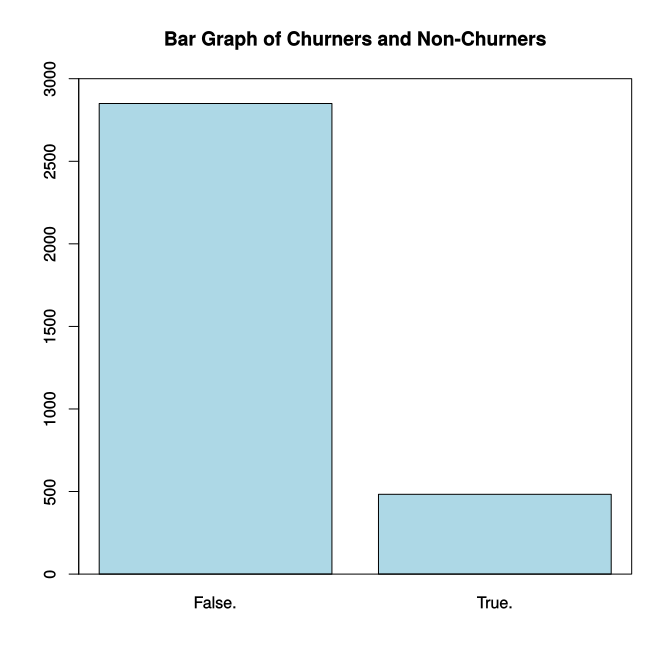
\includegraphics[width=\textwidth]{images/bargraph-churners}
\end{columns}
\end{frame}

\subsection{Churn vs The International Plan}
\begin{frame}{Relating Two Variables}
\begin{columns}
\column{0.5\textwidth}
    \begin{block}{Contingency Table}
        \begin{tabular}{r|r|r}
        & \multicolumn{2}{c}{\bf International Plan} \\
        {\bf Churn} & no & yes \\
        \hline
        False. & 2664 & 186 \\
        True. & 346 & 137 \\
        \end{tabular}
    \end{block}
    \begin{block}{Proportional Contingency Table}
        \begin{tabular}{r|r|r}
        & \multicolumn{2}{c}{\bf International Plan} \\
        {\bf Churn} & no & yes \\
        \hline
        False. & 93.47\% & 6.53\% \\
        True. & 71.64\% & 28.36\% \\
        \end{tabular}
    \end{block}
\column{0.5\textwidth}
    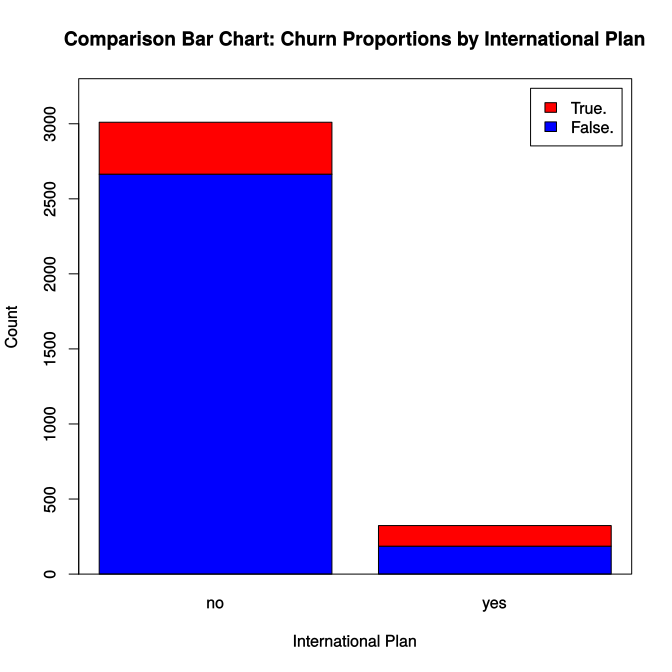
\includegraphics[width=\textwidth]{images/overlay-churn-international}
\end{columns}
\end{frame}


\begin{frame}{Overlayed Bar Chart}
    \centering
    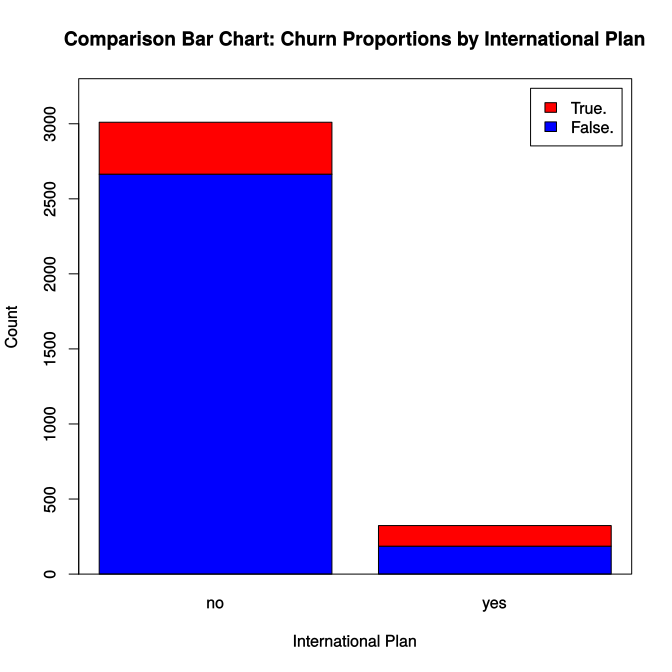
\includegraphics[height=\textheight]{images/overlay-churn-international}
\end{frame}

\begin{frame}{Clustered Bar Chart by International Plan}
    \centering
    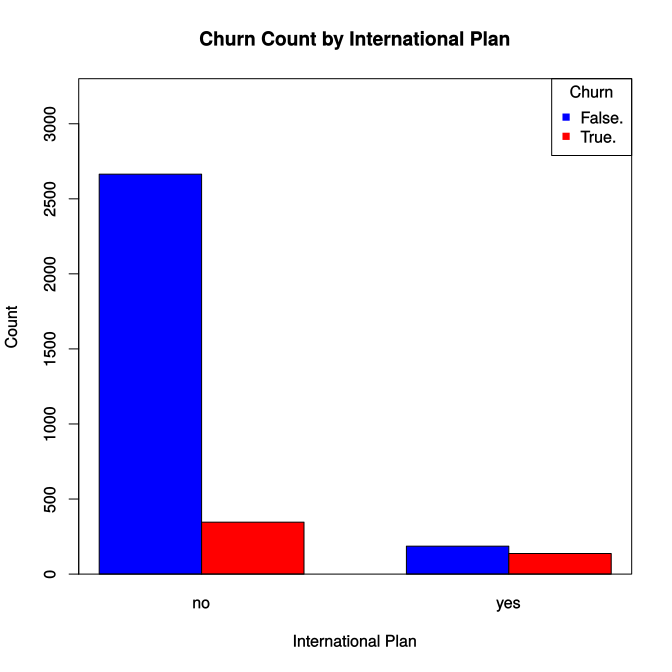
\includegraphics[height=\textheight]{images/cluster-by-international}
\end{frame}

\begin{frame}{Clustered Bar Chart by Churn}
    \centering
    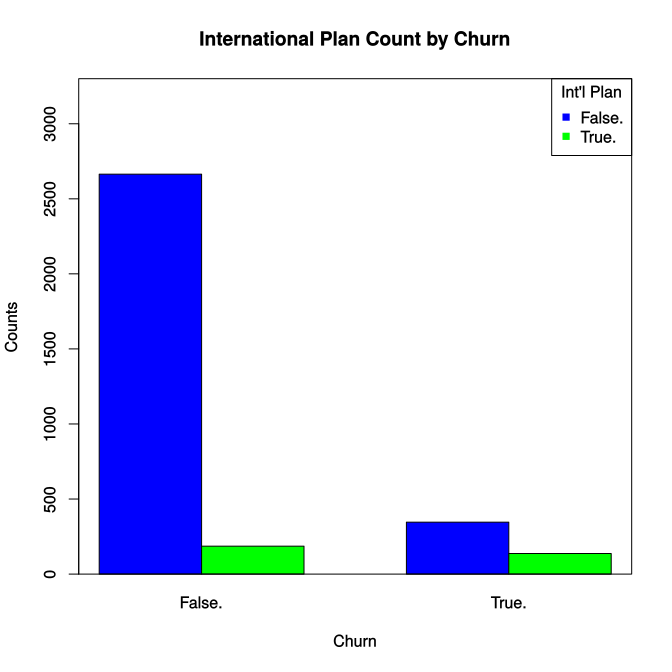
\includegraphics[height=0.8\textheight]{images/cluster-by-churn}
\end{frame}

\subsection{Churn and Customer Service Calls}
\begin{frame}{Histogram of Customer Service Calls}
    \centering
    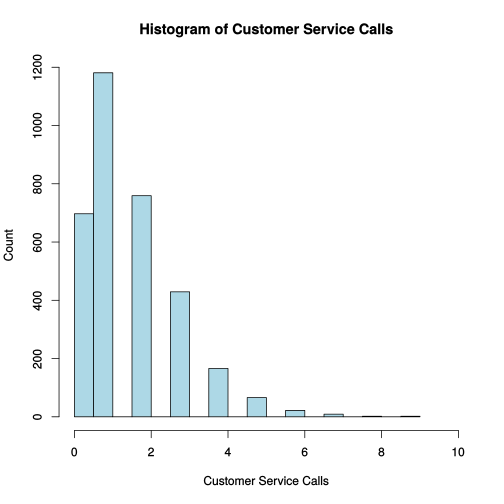
\includegraphics[height=0.8\textheight]{images/hist-customer-calls}
\end{frame}

\begin{frame}{Overlay of Customer Service Calls and Churn}
    \centering
    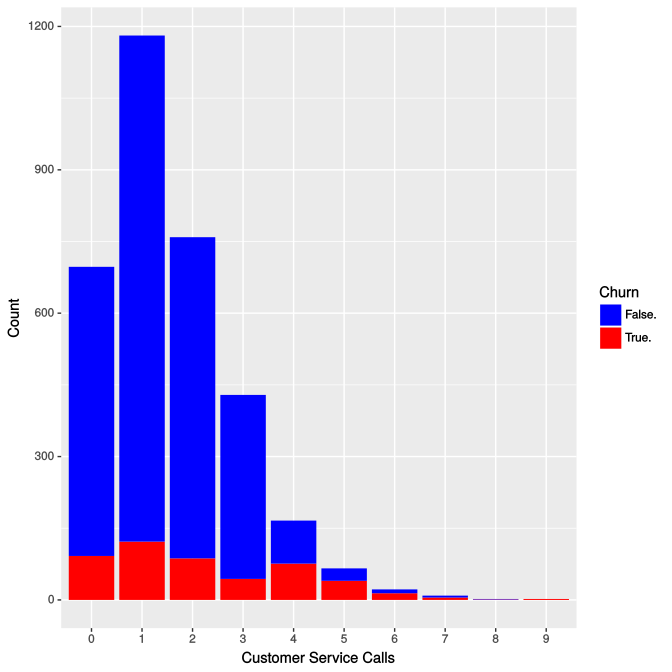
\includegraphics[height=0.8\textheight]{images/overlay-customer-calls}    
\end{frame}

\begin{frame}{Overlay of Customer Service Calls and Churn Percent}
    \centering
    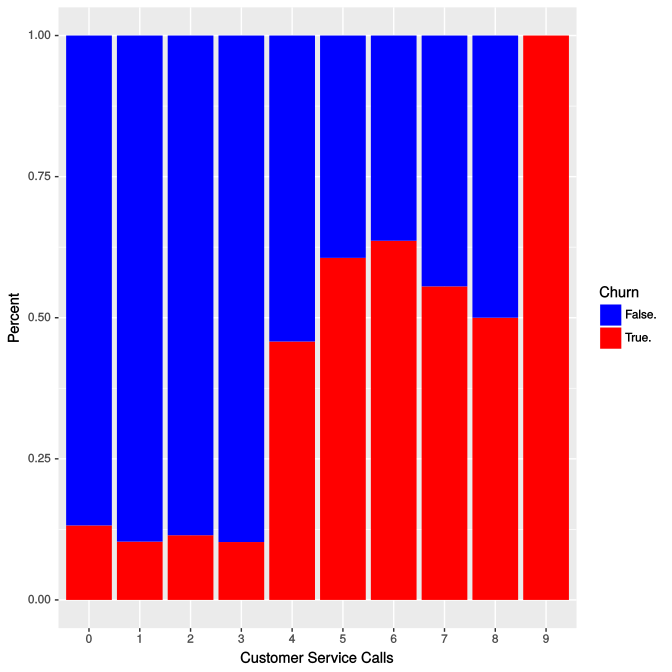
\includegraphics[height=0.8\textheight]{images/overlay-customer-calls-percent}
\end{frame}

\subsection{Churn and Minutes}
\begin{frame}{Scatter Plot of Day Minutes, Evening Minutes, and Churn}
    \centering
    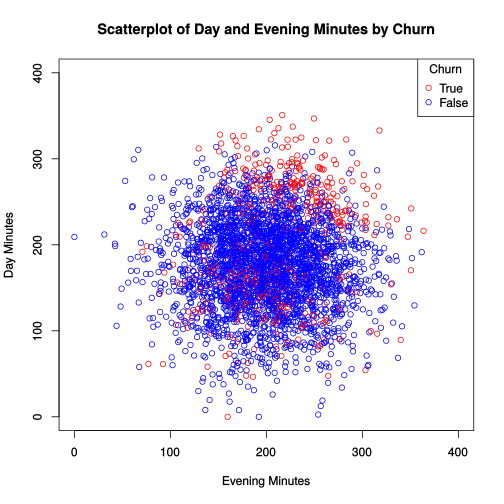
\includegraphics[height=0.8\textheight]{images/scatter-minutes}
\end{frame}

\begin{frame}{Scatter Plot of Customer Calls, Day Minutes, and Churn}
    \centering
    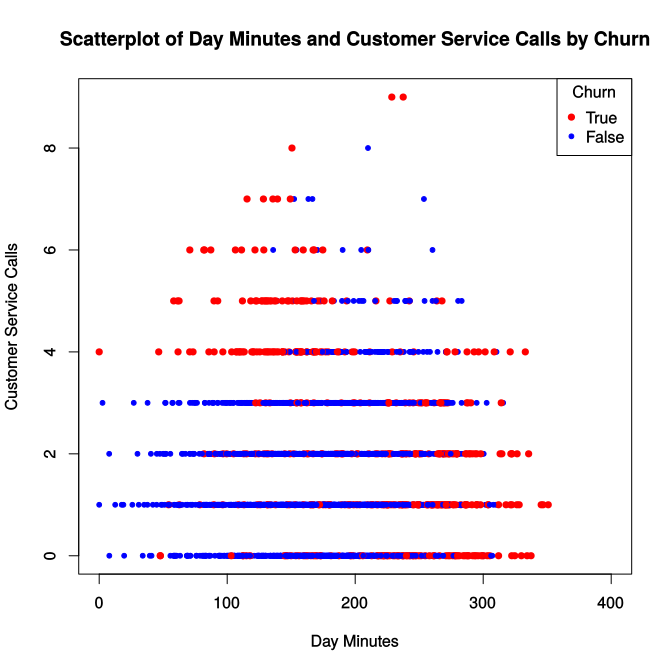
\includegraphics[height=0.8\textheight]{images/scatter-minutes-calls}
\end{frame}

\section{Homework}
\end{document}


